\documentclass[]{elsarticle} %review=doublespace preprint=single 5p=2 column
%%% Begin My package additions %%%%%%%%%%%%%%%%%%%
\usepackage[hyphens]{url}

  \journal{An awesome journal} % Sets Journal name


\usepackage{lineno} % add
\providecommand{\tightlist}{%
  \setlength{\itemsep}{0pt}\setlength{\parskip}{0pt}}

\usepackage{graphicx}
\usepackage{booktabs} % book-quality tables
%%%%%%%%%%%%%%%% end my additions to header

\usepackage[T1]{fontenc}
\usepackage{lmodern}
\usepackage{amssymb,amsmath}
\usepackage{ifxetex,ifluatex}
\usepackage{fixltx2e} % provides \textsubscript
% use upquote if available, for straight quotes in verbatim environments
\IfFileExists{upquote.sty}{\usepackage{upquote}}{}
\ifnum 0\ifxetex 1\fi\ifluatex 1\fi=0 % if pdftex
  \usepackage[utf8]{inputenc}
\else % if luatex or xelatex
  \usepackage{fontspec}
  \ifxetex
    \usepackage{xltxtra,xunicode}
  \fi
  \defaultfontfeatures{Mapping=tex-text,Scale=MatchLowercase}
  \newcommand{\euro}{€}
\fi
% use microtype if available
\IfFileExists{microtype.sty}{\usepackage{microtype}}{}
\bibliographystyle{elsarticle-harv}
\ifxetex
  \usepackage[setpagesize=false, % page size defined by xetex
              unicode=false, % unicode breaks when used with xetex
              xetex]{hyperref}
\else
  \usepackage[unicode=true]{hyperref}
\fi
\hypersetup{breaklinks=true,
            bookmarks=true,
            pdfauthor={},
            pdftitle={Changes in accessibility to foodbanks during COVID-19 and implications for the food security of vulnerable populations in Hamilton, Ontario},
            colorlinks=false,
            urlcolor=blue,
            linkcolor=magenta,
            pdfborder={0 0 0}}
\urlstyle{same}  % don't use monospace font for urls

\setcounter{secnumdepth}{0}
% Pandoc toggle for numbering sections (defaults to be off)
\setcounter{secnumdepth}{0}

% Pandoc citation processing
\newlength{\csllabelwidth}
\setlength{\csllabelwidth}{3em}
\newlength{\cslhangindent}
\setlength{\cslhangindent}{1.5em}
% for Pandoc 2.8 to 2.10.1
\newenvironment{cslreferences}%
  {}%
  {\par}
% For Pandoc 2.11+
\newenvironment{CSLReferences}[3] % #1 hanging-ident, #2 entry spacing
 {% don't indent paragraphs
  \setlength{\parindent}{0pt}
  % turn on hanging indent if param 1 is 1
  \ifodd #1 \everypar{\setlength{\hangindent}{\cslhangindent}}\ignorespaces\fi
  % set entry spacing
  \ifnum #2 > 0
  \setlength{\parskip}{#2\baselineskip}
  \fi
 }%
 {}
\usepackage{calc} % for calculating minipage widths
\newcommand{\CSLBlock}[1]{#1\hfill\break}
\newcommand{\CSLLeftMargin}[1]{\parbox[t]{\csllabelwidth}{#1}}
\newcommand{\CSLRightInline}[1]{\parbox[t]{\linewidth - \csllabelwidth}{#1}}
\newcommand{\CSLIndent}[1]{\hspace{\cslhangindent}#1}

% Pandoc header
\usepackage{booktabs}
\usepackage{longtable}
\usepackage{array}
\usepackage{multirow}
\usepackage{wrapfig}
\usepackage{float}
\usepackage{colortbl}
\usepackage{pdflscape}
\usepackage{tabu}
\usepackage{threeparttable}
\usepackage{threeparttablex}
\usepackage[normalem]{ulem}
\usepackage{makecell}
\usepackage{xcolor}



\begin{document}
\begin{frontmatter}

  \title{Changes in accessibility to foodbanks during COVID-19 and
implications for the food security of vulnerable populations in
Hamilton, Ontario}
    \author[Some University]{Author One\corref{1}}
   \ead{author1@example.com} 
    \author[]{Author Two}
   \ead{author2@example.com} 
    \author[Some University]{Author Three\corref{2}}
   \ead{author3@example.com} 
    \author[Another University]{Author Four\corref{2}}
   \ead{author4@example.com} 
      \address[Some University]{Department, Street, City, State, Zip}
    \address[Another University]{Department, Street, City, State, Zip}
      \cortext[1]{Corresponding Author}
    \cortext[2]{Equal contribution}
  
  \begin{abstract}
  This is the abstract.

  It consists of two paragraphs.
  \end{abstract}
  
 \end{frontmatter}

\hypertarget{credit-author-statement}{%
\section{CRediT author statement}\label{credit-author-statement}}

\textbf{Author 1:} Conceptualization, Methodology, Software, Validation,
Formal analysis, Investigation, Data Curation, Writing - Original Draft,
Visualization, Supervision; \textbf{Author 2:} Conceptualization,
Methodology, Software, Validation, Formal analysis, Investigation, Data
Curation, Writing - Original Draft, Visualization; \textbf{Author 3:}
Conceptualization, Investigation, Data Curation, Writing - Original
Draft; \textbf{Author 4:} Resources - Writing: Review \& Editing -
Supervision

\newpage

\hypertarget{introduction}{%
\section{Introduction}\label{introduction}}

Food insecurity, defined as an ``inadequate or uncertain access to a
sufficient quantity and/or adequate quality of food'' due to a
household's financial limitations (Enns et al., 2020), has been
associated with reductions in nutritional outcomes (Bhattacharya et al.,
2004; Kirkpatrick and Tarasuk, 2008; Olson, 1999) and physical and
mental health in children and adults (Elgar et al., 2021; Jones, 2017;
Ramsey et al., 2011; Seligman et al., 2010; Stuff et al., 2004). Over at
least the past four decades food banks have become an essential line of
defense against food insecurity in Canadian communities (Black and Seto,
2020; Holmes et al., 2018; Riches, 2002; Tarasuk et al., 2020). In this
respect, Canada is not unlike numerous other wealthy countries where a
systematic dismantling of the welfare state took place in the
intervening period (Tarasuk et al., 2014).

But the emergence of COVID-19, the worst public health crisis since the
1918 flu pandemic, has revealed important social and economic fault
lines, and pre-existing patterns of inequality appear to have been
exacerbated. Along several other dimensions of stress {[}e.g.,
accessibility to health care facilities; Pereira et al. (2021a){]}, this
seems to be the case for food insecurity as well (Laborde et al., 2020).
In the US, for example, it has been estimated that there was an increase
of more than 30\% in household food insecurity, and more than one third
of households were discovered to be newly food insecure - meaning they
did not experience food insecurity before the pandemic (Niles et al.,
2020). In Canada, Men and Tarasuk (2021) report that about 25\% of
individuals who experienced job insecurity (a relatively common
occurrence during the pandemic), also experienced food insecurity.
Similarly, according to Statistics Canada (2020a), in the early stages
of the pandemic almost 15\% of individuals reported living in a
household that faced food insecurity; the risk of food insecurity was
substantially higher for households with children. The difference
between households with and without children was significant, and 11.7\%
of households with children indicated that ``food didn't last and
{[}there was{]} no money to get more'' sometimes or often, compared to
7.3\% of households without children); likewise, 13\% of households with
children indicated that they ``{[}c{]}ouldn't afford balanced meals''
sometimes or often, compared to 8.8\% of households without children.

The impacts of food insecurity during the pandemic are alarming, since
diet-related diseases, such as obesity, heart-disease, and diabetes,
were already critical public health concerns in Canada prior to COVID-19
(Boucher et al., 2017). While food banks are not necessarily a stable
solution to food insecurity and in fact may encourage a retrenchment of
neoliberal policy (Wakefield et al., 2013), at least they can be argued
to provide a resource of last instance to households in precarious
situations (Bazerghi et al., 2016). As recently as 2019, the Hamilton
Hunger Report\footnote{https://www.hamiltonfoodshare.org/wp-content/uploads/Hamilton-Food-Share-Hunger-Report-2019.pdf}
noted that food banks in Hamilton, Ontario, recorded the highest number
of visitors in the past 29 years; the number of children visiting food
banks (minors up to 18 years old) was 9,125 in March 2019, up from 8,278
the year before.

It is known that the urban food environment, within which people make
their daily food choices, is essential in influencing eating behaviours
and health outcomes, based on factors such as food availability, ease of
geographic accessibility and socio-demographic variations (Paez et al.,
2010; Vanderlee and L'Abbé, 2017; Widener, 2018). However, while there
is a wealth of literature that has examined the topic of geographic
accessibility to healthy food through the ``food desert'' concept, there
has been little research into accessibility to food banks. Although
previous work has explored differences in \emph{accessing} food banks,
such as how some households utilize food banks over short periods of
time while others regularly utilize food banks as longer-term resource
(e.g., Enns et al., 2020), we are not aware of any research that has
focused on the geographic component of accessibility. \textbf{Check
Tarasuk et al. (2019)}

The study of place-based geographic accessibility is concerned with
capturing the potential to reach destinations of value using the
transportation network (Páez et al., 2012). Indeed, the Government of
Canada's recent Food Policy has made ``access'' to healthy food a
priority for Canadian communities\footnote{https://www.agr.gc.ca/eng/about-our-department/key-departmental-initiatives/food-policy/the-food-policy-for-canada/?id=1597863791042}
and previous survey research has suggested that such accessibility plays
a key role in user satisfaction with food bank service delivery in
Vancouver (Holmes et al., 2018). However, as with research into the
prevalence of food deserts, accessibility to food banks is likely not
evenly distributed throughout a city with variations in access
attributable to transportation network characteristics and the spatial
distribution of food bank locations - as well as the population that
likely needs them. Furthermore, policy responses to the COVID-19
pandemic add to the distress of vulnerable households.
Non-pharmaceutical interventions during the pandemic involving
restrictions in mobility increased the friction of travel, in particular
by transit on which low income populations are more likely to be reliant
(e.g., DeWeese et al., 2020). At the same time, the pandemic has created
additional stress for the operators of foodbanks through disruptions in
the supply chain (e.g., McKay et al., 2021) as well as concerns
surrounding the delivery of service in safe conditions and possible
cancellation of food service programs.

For this study, we aim to look at how the landscape of food banks and
related services (e.g.~low-cost or free meal service providers)
available in Hamilton, Ontario, has changed before and during the
pandemic. Have the number of open food bank services diminished? If so,
what was the accessibility to foodbanks before and during the pandemic,
from the perspective of low income households? And finally, who are most
likely to have been impacted by changes to the accessibility landscape?
This paper will first look at the distribution of food banks and related
services before and during the pandemic. Then, we use the balanced
floating catchment area approach of Paez et al. (Paez et al., 2019) to
investigate the accessibility situation. We use a fully disaggregated
approach based on parcel-level data. Socio-economic and demographic data
are drawn from the latest Census of Canada (2016), whereas travel
information is from the most recent regional travel survey from 2016.
This paper follows reproducible research recommendations (see Brunsdon
and Comber, 2020), and the research was conducted using open source
tools for transportation analysis (Lovelace, 2021). The code and data
necessary to reproduce the analysis are available in a public
repository\footnote{add repository}.

\hypertarget{literature-review}{%
\section{Literature Review}\label{literature-review}}

\hypertarget{food-insecurity}{%
\subsection{Food Insecurity}\label{food-insecurity}}

Food insecurity is the inability to acquire and consume an adequate
amount or good quality food, leading to inadequate nutrient intake
(Kirkpatrick and Tarasuk, 2008; Tarasuk and Vogt, 2009). This nutrient
deficiency has been causing major health concerns in Canadians, and
particularly those who are at a socioeconomic disadvantage (Bazerghi et
al., 2016). Previous studies have aimed to look at the relationship
between the built food environment and socio-demographic characteristics
with qualitative and quantitative, or a mixed -method approach.
Quantitatively, official governmental surveys have been able to assist
with data, such as the Household Food Security Survey Module (HFSSM),
the Canadian Community Health Surveys (CCHS), the Longitudinal and
International Study of Adults (LISA), and official classifications
determined by Health Canada in relation to sociodemographic variables
(Gundersen et al., 2018; Kirkpatrick and Tarasuk, 2008; Tarasuk and
Vogt, 2009). Studies have also aimed to assess food availability of
healthy foods (e.g., fruit and vegetables) at supermarkets in relation
to sociodemographic characteristics and geographic accessibility (Latham
and Moffat, 2007). In terms of findings, studies have generated
inconsistent relationships between their evaluated availability of food
and sociodemographic characteristics that go in hand.

\hypertarget{foodbanks}{%
\subsection{Foodbanks}\label{foodbanks}}

Food banks - sometimes also referred to as `food pantries' and `food
shelves' - originated as a community response to aid those with
inadequate food by voluntarily offering them meals and ingredients
(Loopstra and Tarasuk, 2012; Riches, 2002). The scope and objectives of
foodbanks can vary by region and by country, and these organizations can
include not only prepared meals and aliments, but also shared spaces to
connect in community gardens and community kitchens (Wakefield et al.,
2013). Although in their origin foodbanks were meant to be provide a
temporary solution to accommodate those in hunger due to job
retrenchments and economic downfalls since the 1980s, over time they
evolved into a community practice to secure emergency food supplies for
those in need (Loopstra and Tarasuk, 2012; Wakefield et al., 2013). In
Canada, the number of foodbanks has steadily increased in the past few
decades (Wakefield et al., 2013). Previous studies have questioned
whether food banks are able to offer a rounded nutritious supply of
food, and if food banks are a sustainable on-going practice for those in
need (Bazerghi et al., 2016; Riches, 2002). An inescapable reality, at
the moment, is that despite their imperfections they provide urgently
needed support for members of the population for whom foodbanks are
frequently their primary location to get food (Bazerghi et al., 2016).
\textbf{However, surveys revealed that only 20 to 30 percent of those
experiencing food insecurity were found to frequent food banks in Canada
(Tarasuk et al., 2014).} \textbf{Something about geographical access}

\hypertarget{food-insecurity-in-canada-during-the-covid-19}{%
\subsection{Food Insecurity in Canada during the
COVID-19}\label{food-insecurity-in-canada-during-the-covid-19}}

Currently with the COVID-19 pandemic, disrupted economies, rising
unemployment rates, and changes in poverty levels have disrupted the
food environment and led to higher rates of food insecurity (Niles et
al., 2020). In 2012, 12.4\% of Canadians households and 11.8\% Ontarian
households experienced some degree of food insecurity (Gundersen et al.,
2018; Tarasuk et al., 2020). Pandemic-related food security studies in
the US have found a substantial increase in households experiencing food
insecurity for the first time, and also in households experiencing more
severe food insecurity than before (Niles et al., 2020; Wolfson and
Leung, 2020). Most recently in May 2020, Canada recorded 14.7\% of its
population living in food insecurity in the past 30 days (Statistics
Canada, 2020a). Food insecurity is a highly concerning public health
issue due to its health impacts. Recent research suggests that food
insecurity in adults can lead to experiencing more stressful events
(El-hajj and Benhin 2021). Increases in food insecurity rates due to the
pandemic, signal a change in the food environment with potential damages
to population health during the course of the pandemic and beyond (Niles
et al., 2020).

\hypertarget{methods-and-materials}{%
\section{Methods and Materials}\label{methods-and-materials}}

\hypertarget{methods}{%
\subsection{Methods}\label{methods}}

For the research in this paper we adopt the balanced floating catchment
area approach of Paez et al. (2019). This method for estimating
accessibility is a form of the common two-stage floating catchment area
method (Luo and Wang, 2003; Radke and Mu, 2000). Floating catchment
areas are used to estimate accessibility when there are potential
congestion effects, and operate by calculating first the \emph{demand}
for spatially distributed services. The demand (usually the number of
people who require a service) is used to calculate a level of service.
In a second step, the level of service is allocated back to the
population. Demand and level of service are allocated using some form of
distance-decay to embody the geographical principle that, given a
choice, people prefer to travel less than more when reaching
destinations.

More formally, the first step of this method is as follows: \[
L_j = \frac{S_j}{\sum_{i=1}^nP_iw_{ij}}
\]

\noindent where \(S_j\) is the level of supply at location \(j\), in
simplest terms whether a service point is present (i.e., \(S_j=1\)) or
not (i.e., \(S_j=0\)); \(P_i\) is the population at location \(i\) that
demands the service; and \(w_{ij}\) is a weight, typically a function of
the distance between locations \(i\) and \(j\). \(L_j\) is the level of
service at location \(j\) and it is the inverse of the number of people
that need to be serviced.

The second step in this process is then summing the level of service
that each population unit can reach, according to the distance-decay
weight: \[
A_i = \sum_{j=1}^JL_jw_{ji}
\]

\noindent where \(A_i\) is the accessibility to the service, which is in
the same units as the level of service: as the inverse of the population
being serviced. When the population being serviced is low accessibility
is high (i.e., there is little competition for the service), and
viceversa.

Floating catchment area methods are prone to overestimation of the
population and the level of service due to multiple-counting. The
population at \(P_i\) is allocated to \emph{every} service point \(j\)
for which \(w_{ij}>0\). Similarly, the level of service at \(LOS_j\) is
allocated to \emph{every} population point for which \(w_{ji}>0\). This
inflation effect has been known for several years, and several
modifications have been proposed to mitigate it (Delamater, 2013; e.g.,
Wan et al., 2012). A definitive solution to this issue was presented by
Paez et al. (2019). In order to avoid the multiple-counting in the
summations, the population and the level of service need to be allocated
\emph{proportionally}. This is achieved by standardizing the weights as
follows: \[
w_{ij}^\text{st} = \frac{w_{ij}}{\sum_{i=1}^nw_{ij}}
\] \noindent and: \[
w_{ji}^\text{st} = \frac{w_{ji}}{\sum_{j=1}^Jw_{ji}}
\]

The standardized weights satisfy the following conditions: \[
\sum_{i=1}^nw_{ij}^\text{st}=1
\]

\noindent and: \[
\sum_{j=1}^Jw_{ji}^\text{st}=1
\]

As a result, the total population (and consequently, the level of
service) are preserved system-wide: \[
\sum_{i=1}^nP_iw_{ij}^\text{st}=P_i
\]

\noindent and also: \[
\sum_{j=1}^JL_jw_{ji}^\text{st}=L_j
\]

\hypertarget{data}{%
\subsection{Data}\label{data}}

Data have been prepared for sharing as a data package\footnote{add
  repository}.

\hypertarget{statistics-canada}{%
\subsubsection{Statistics Canada}\label{statistics-canada}}

Population and income statistics at the level of Dissemination Areas
(DAs) were retrieved using the package \texttt{cancensus} (von Bergmann
et al., 2021). Dissemination Areas are the smallest publicly available
census geography in Canada. We use data from the 2016 Population Census.

\hypertarget{origins-residential-parcels}{%
\subsubsection{Origins: Residential
parcels}\label{origins-residential-parcels}}

We converted all recorded residential parcels in the City of Hamilton to
points on the road network. Each point includes information about the
number of residential units in the parcel. Each residential unit is
``populated'' with the probability of being a ``low income household,''
which we define as having a total household income of less than CAD
40,000. This is approximately the mid-point of the low income cut-off
(LICOs) for families in Canadian cities with populations greater than
500,000 in 2016, to match other Census data (Statistics Canada, 2020b).

\hypertarget{destinations-foodbanks}{%
\subsubsection{Destinations: Foodbanks}\label{destinations-foodbanks}}

\textbf{The locations of foodbanks were obtained from public records and
geocoded. Three urban sites not in the program were also identified and
geocoded for comparison purposes.}

\hypertarget{routing-and-travel-time-tables}{%
\subsubsection{Routing and travel time
tables}\label{routing-and-travel-time-tables}}

Travel time tables for three modes (car, transit, walking) were computed
using the parcels as the origins and the locations of the foodbanks as
the destinations. For routing, the package \texttt{r5r} (Pereira et al.,
2021b) was used, with a network extract for the City of Hamilton from
OpenStreetMaps and the General Transit Feed Specification from Hamilton
Street Railway, the local transit operator. For routing purposes we used
maximum values of 180 min and 10,000 m walking distance: any destination
that exceeded these thresholds was ignored. The departure time used for
routing was \textbf{TIME}.

\hypertarget{open-hamilton}{%
\subsubsection{\texorpdfstring{Open Hamilton
\textbf{???}}{Open Hamilton ???}}\label{open-hamilton}}

We used the open data portal of the City of
Hamilton\footnote{\url{https://open.hamilton.ca/}} we obtained
boundaries for the city's various regions (the definition of urban,
suburban, and rural regions follows the classification of development
applications).

\hypertarget{transportation-tomorrow-survey}{%
\subsubsection{Transportation Tomorrow
Survey}\label{transportation-tomorrow-survey}}

We used the Data Retrieval System of the Transportation Tomorrow Survey
(TTS)\footnote{\url{http://dmg.utoronto.ca/}} to download
cross-tabulations of: 1) primary mode of travel per trip by income by
place of residence; and 2) age by income by place of residence. These
data are from the 2016 Survey (the most recent available), and data are
geocoded at the level of Traffic Analysis Zones (TAZ) using the most
recent zoning system from 2006. Each parcel point is populated with the
proportion of trips by three modes of travel: car (as driver or
passenger), transit, and walk.

\hypertarget{expected-travel-times}{%
\subsubsection{Expected Travel Times}\label{expected-travel-times}}

Once we obtained travel time tables with population (number of
households) and proportion of trips by mode, we calculated the expected
travel time \(ett\) from each parcel \(i\) to a foodbank \(j\) as
follows: \[
ett_i = p^c_i\cdot tt^c_{ij} + p^t_i\cdot tt^t_{ij} + p^w_i\cdot tt^w_{ij}
\] \noindent where \(p^k_i\) is the proportion of trips by mode \(k\) in
the TAZ of parcel \(i\), and \(tt^k_{ij}\) is the travel time from
parcel \(i\) to the foodbank. In other words, the expected travel time
is the weighted sum of travel times to the foodbank, with the weights
given by the expected modal split in the TAZ.

\hypertarget{results-and-discussion}{%
\section{Results and Discussion}\label{results-and-discussion}}

Words go here.

\begin{figure}
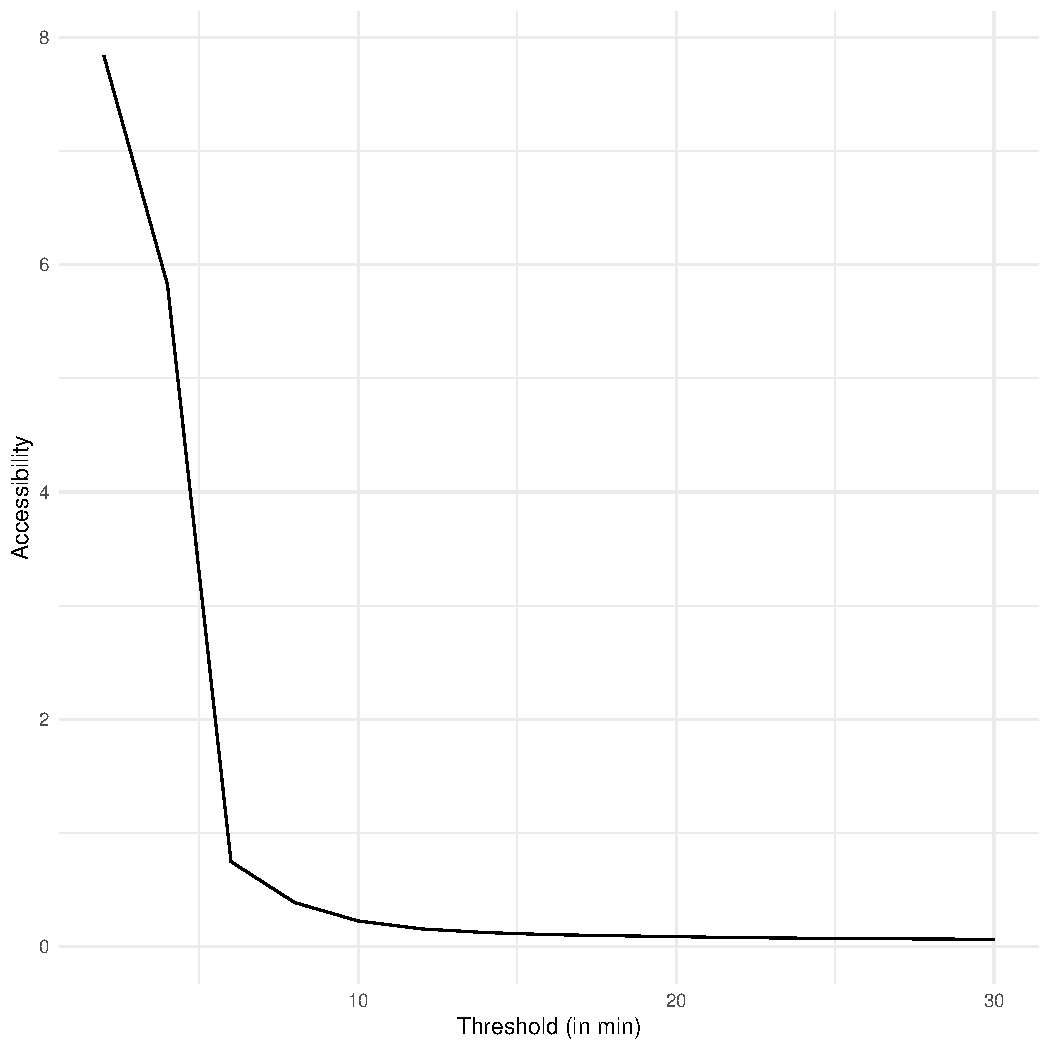
\includegraphics[width=0.9\linewidth]{Accessibility-Foodbanks-Hamilton_files/figure-latex/plot-results-sensitivity-analysis-1} \caption{\label{fig:sensitivity-analysis}Accessibility as a function of threshold}\label{fig:plot-results-sensitivity-analysis}
\end{figure}

\begin{table}

\caption{\label{tab:table-accessibility-by-age-group}\label{tab:accessibility-by-age}Accessibility by age group among members of low income households.}
\centering
\resizebox{\linewidth}{!}{
\begin{tabular}[t]{cccccc}
\toprule
\multicolumn{3}{c}{Population} & \multicolumn{3}{c}{Accessibility} \\
\cmidrule(l{3pt}r{3pt}){1-3} \cmidrule(l{3pt}r{3pt}){4-6}
Children (age $\le$ 18) & Adults (19-64) & Seniors (age $\ge$ 65) & Before COVID-19 & During COVID-19 & Difference\\
\midrule
\cellcolor{gray!6}{7,015} & \cellcolor{gray!6}{21,586} & \cellcolor{gray!6}{9,158} & \cellcolor{gray!6}{0.00734} & \cellcolor{gray!6}{0.00438} & \cellcolor{gray!6}{-0.00296}\\
3,490 & 13,598 & 6,618 & 0.01386 & 0.00812 & -0.00575\\
\cellcolor{gray!6}{966} & \cellcolor{gray!6}{5,180} & \cellcolor{gray!6}{4,310} & \cellcolor{gray!6}{0.01475} & \cellcolor{gray!6}{0.00849} & \cellcolor{gray!6}{-0.00625}\\
2,384 & 7,725 & 5,595 & 0.01853 & 0.01079 & -0.00775\\
\bottomrule
\multicolumn{6}{l}{\rule{0pt}{1em}\textit{Note: }}\\
\multicolumn{6}{l}{\rule{0pt}{1em}Population values have been rounded}\\
\end{tabular}}
\end{table}

\begin{figure}
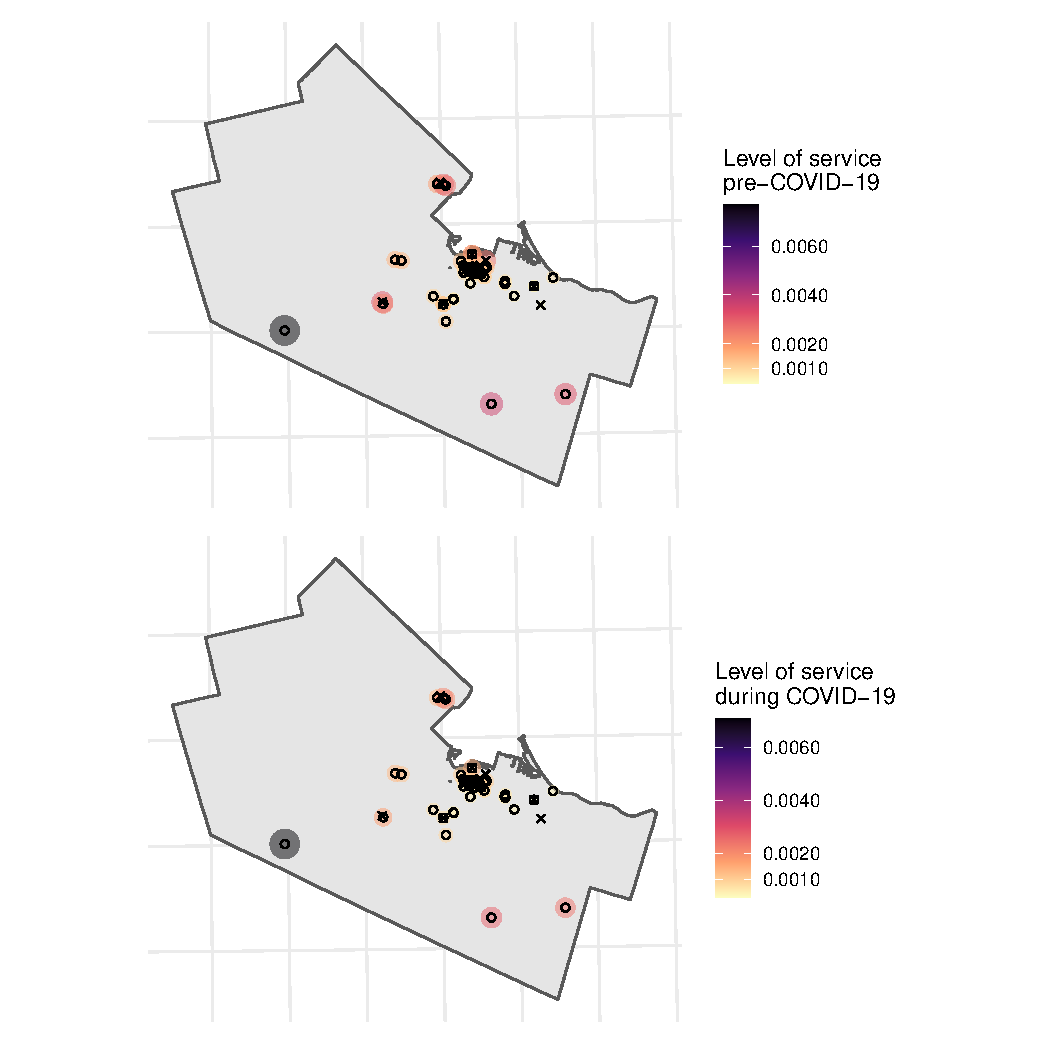
\includegraphics[width=0.9\linewidth]{Accessibility-Foodbanks-Hamilton_files/figure-latex/plot-levels-of-service-1} \caption{\label{fig:levels-of-service}Levels of service at each facility pre-COVID-19 (top panel) and during COVID-19 (middle panel). The bottom panel shows the change in level of service.}\label{fig:plot-levels-of-service}
\end{figure}

\begin{figure}

{\centering 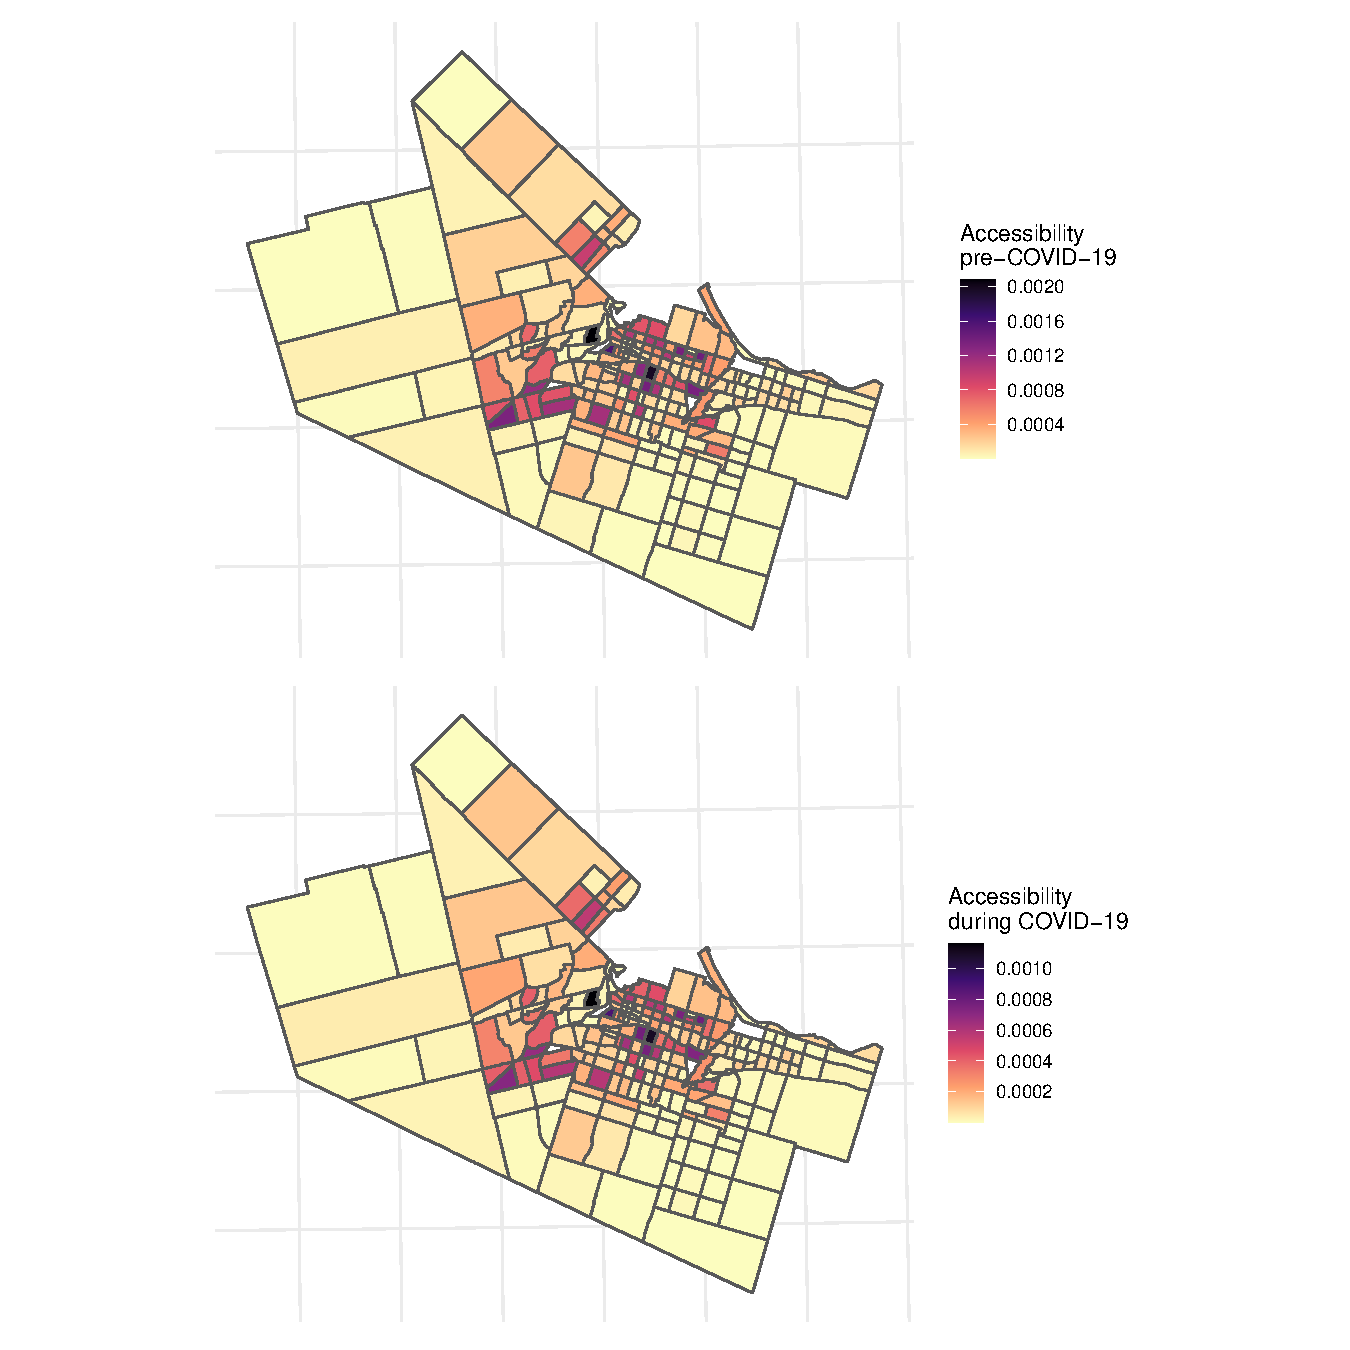
\includegraphics[width=0.9\linewidth]{Accessibility-Foodbanks-Hamilton_files/figure-latex/plot-accessibility-1} 

}

\caption{\label{fig:accessibility}Accessibility by traffic analysis zone pre-COVID-19 (top panel) and during COVID-19 (middle panel). The bottom panel shows the change in accessibility.}\label{fig:plot-accessibility}
\end{figure}

\hypertarget{conclusions}{%
\section{Conclusions}\label{conclusions}}

Words go here.

\hypertarget{references}{%
\section*{References}\label{references}}
\addcontentsline{toc}{section}{References}

\hypertarget{refs}{}
\begin{CSLReferences}{1}{0}
\leavevmode\hypertarget{ref-bazerghi2016role}{}%
Bazerghi, C., McKay, F.H., Dunn, M., 2016. The role of food banks in
addressing food insecurity: A systematic review. Journal of community
health 41, 732--740.

\leavevmode\hypertarget{ref-bhattacharya2004poverty}{}%
Bhattacharya, J., Currie, J., Haider, S., 2004. Poverty, food
insecurity, and nutritional outcomes in children and adults. Journal of
health economics 23, 839--862.
doi:\url{https://doi.org/10.1016/j.jhealeco.2003.12.008}

\leavevmode\hypertarget{ref-black2020examining}{}%
Black, J.L., Seto, D., 2020. Examining patterns of food bank use over
twenty-five years in vancouver, canada. VOLUNTAS: International Journal
of Voluntary and Nonprofit Organizations 31, 853--869.
doi:\url{https://doi.org/10.1007/s11266-018-0039-2}

\leavevmode\hypertarget{ref-boucher2017ontario}{}%
Boucher, B.A., Manafò, E., Boddy, M.R., Roblin, L., Truscott, R., 2017.
The ontario food and nutrition strategy: Identifying indicators of food
access and food literacy for early monitoring of the food environment.
Health promotion and chronic disease prevention in Canada : research,
policy and practice 37, 313--319.
doi:\href{https://doi.org/10.24095/hpcdp.37.9.06}{10.24095/hpcdp.37.9.06}

\leavevmode\hypertarget{ref-brunsdon2020opening}{}%
Brunsdon, C., Comber, A., 2020. Opening practice: Supporting
reproducibility and critical spatial data science. Journal of
Geographical Systems 1--20.
doi:\href{https://doi.org/10.1007/s10109-020-00334-2}{10.1007/s10109-020-00334-2}

\leavevmode\hypertarget{ref-delamater2013spatial}{}%
Delamater, P.L., 2013. Spatial accessibility in suboptimally configured
health care systems: A modified two-step floating catchment area
(M2SFCA) metric. Health \& Place 24, 30--43.
doi:\href{https://doi.org/10.1016/j.healthplace.2013.07.012}{10.1016/j.healthplace.2013.07.012}

\leavevmode\hypertarget{ref-deweese2020tale}{}%
DeWeese, J., Hawa, L., Demyk, H., Davey, Z., Belikow, A., El-geneidy,
A., 2020. A tale of 40 cities: A preliminary analysis of equity impacts
of COVID-19 service adjustments across north america. Findings.
doi:\href{https://doi.org/10.32866/001c.13395}{10.32866/001c.13395}

\leavevmode\hypertarget{ref-elgar2021relative}{}%
Elgar, F.J., Pickett, W., Pförtner, T.-K., Gariépy, G., Gordon, D.,
Georgiades, K., Davison, C., Hammami, N., MacNeil, A.H., Da Silva, M.A.,
others, 2021. Relative food insecurity, mental health and wellbeing in
160 countries. Social Science \& Medicine 268, 113556.
doi:\url{https://doi.org/10.1016/j.socscimed.2020.113556}

\leavevmode\hypertarget{ref-enns2020experiences}{}%
Enns, A., Rizvi, A., Quinn, S., Kristjansson, E., 2020. Experiences of
food bank access and food insecurity in ottawa, canada. Journal of
Hunger \& Environmental Nutrition 15, 456--472.
doi:\url{https://doi.org/10.1080/19320248.2020.1761502}

\leavevmode\hypertarget{ref-gundersen2018food}{}%
Gundersen, C., Tarasuk, V., Cheng, J., De Oliveira, C., Kurdyak, P.,
2018. Food insecurity status and mortality among adults in ontario,
canada. PloS one 13, e0202642.

\leavevmode\hypertarget{ref-holmes2018nothing}{}%
Holmes, E., Black, J.L., Heckelman, A., Lear, S.A., Seto, D., Fowokan,
A., Wittman, H., 2018. {``Nothing is going to change three months from
now''}: A mixed methods characterization of food bank use in greater
vancouver. Social Science \& Medicine 200, 129--136.
doi:\url{https://doi.org/10.1016/j.socscimed.2018.01.029}

\leavevmode\hypertarget{ref-jones2017food}{}%
Jones, A.D., 2017. Food insecurity and mental health status: A global
analysis of 149 countries. American journal of preventive medicine 53,
264--273. doi:\url{https://doi.org/10.1016/j.amepre.2017.04.008}

\leavevmode\hypertarget{ref-kirkpatrick2008food}{}%
Kirkpatrick, S.I., Tarasuk, V., 2008. Food insecurity is associated with
nutrient inadequacies among canadian adults and adolescents. The Journal
of nutrition 138, 604--612.
doi:\url{https://doi.org/10.1093/jn/138.7.1399}

\leavevmode\hypertarget{ref-laborde2020poverty}{}%
Laborde, D., Martin, W., Vos, R., 2020. Poverty and food insecurity
could grow dramatically as COVID-19 spreads. International Food Policy
Research Institute (IFPRI), Washington, DC.

\leavevmode\hypertarget{ref-latham2007determinants}{}%
Latham, J., Moffat, T., 2007. Determinants of variation in food cost and
availability in two socioeconomically contrasting neighbourhoods of
hamilton, ontario, canada. Health \& Place 13, 273--287.
doi:\url{https://doi.org/10.1016/j.healthplace.2006.01.006}

\leavevmode\hypertarget{ref-loopstra2012relationship}{}%
Loopstra, R., Tarasuk, V., 2012. The relationship between food banks and
household food insecurity among low-income toronto families. Canadian
Public Policy 38, 497--514.
doi:\href{https://doi.org/10.3138/cpp.38.4.497}{10.3138/cpp.38.4.497}

\leavevmode\hypertarget{ref-lovelace2021open}{}%
Lovelace, R., 2021. Open source tools for geographic analysis in
transport planning. Journal of Geographical Systems.
doi:\href{https://doi.org/10.1007/s10109-020-00342-2}{10.1007/s10109-020-00342-2}

\leavevmode\hypertarget{ref-luo2003measures}{}%
Luo, W., Wang, F.H., 2003. Measures of spatial accessibility to health
care in a GIS environment: Synthesis and a case study in the chicago
region. Environment and Planning B-Planning \& Design 30, 865--884.

\leavevmode\hypertarget{ref-mckay2021exploring}{}%
McKay, F.H., Bastian, A., Lindberg, R., 2021. Exploring the response of
the victorian emergency and community food sector to the COVID-19
pandemic. Journal of Hunger \& Environmental Nutrition 1--15.
doi:\href{https://doi.org/10.1080/19320248.2021.1900974}{10.1080/19320248.2021.1900974}

\leavevmode\hypertarget{ref-men2021food}{}%
Men, F., Tarasuk, V., 2021. Food insecurity amid the COVID-19 pandemic:
Food charity, government assistance and employment. Canadian Public
Policy COVID-19, e2021001.
doi:\href{https://doi.org/10.3138/cpp.2021-001}{10.3138/cpp.2021-001}

\leavevmode\hypertarget{ref-niles2020early}{}%
Niles, M.T., Bertmann, F., Belarmino, E.H., Wentworth, T., Biehl, E.,
Neff, R., 2020. The early food insecurity impacts of COVID-19. Nutrients
12, 2096.

\leavevmode\hypertarget{ref-olson1999nutrition}{}%
Olson, C.M., 1999. Nutrition and health outcomes associated with food
insecurity and hunger. The Journal of nutrition 129, 521S--524S.
doi:\url{https://doi.org/10.1093/jn/129.2.521S}

\leavevmode\hypertarget{ref-paez2019demand}{}%
Paez, A., Higgins, C.D., Vivona, S.F., 2019. Demand and level of service
inflation in floating catchment area (FCA) methods. PloS one 14,
e0218773.
doi:\href{https://doi.org/10.1371/journal.pone.0218773}{10.1371/journal.pone.0218773}

\leavevmode\hypertarget{ref-paez2010relative}{}%
Paez, A., Mercado, R.G., Farber, S., Morency, C., Roorda, M., 2010.
Relative accessibility deprivation indicators for urban settings:
Definitions and application to food deserts in montreal. Urban Studies
47, 1415--1438.
doi:\href{https://doi.org/10.1177/0042098009353626}{10.1177/0042098009353626}

\leavevmode\hypertarget{ref-paez2012measuring}{}%
Páez, A., Scott, D.M., Morency, C., 2012. Measuring accessibility:
Positive and normative implementations of various accessibility
indicators. Journal of Transport Geography 25, 141--153.
doi:\url{https://doi.org/10.1016/j.jtrangeo.2012.03.016}

\leavevmode\hypertarget{ref-pereira2021geographic}{}%
Pereira, R.H.M., Braga, C.K.V., Servo, L.M., Serra, B., Amaral, P.,
Gouveia, N., Paez, A., 2021a. Geographic access to COVID-19 healthcare
in brazil using a balanced float catchment area approach. Social Science
\& Medicine 273, 113773.
doi:\url{https://doi.org/10.1016/j.socscimed.2021.113773}

\leavevmode\hypertarget{ref-pereira2021r5r}{}%
Pereira, R.H.M., Saraiva, M., Herszenhut, D., Braga, C.K.V., Conway,
M.W., 2021b. r5r: Rapid realistic routing on multimodal transport
networks with r\textsuperscript{5} in r. Findings.
doi:\href{https://doi.org/10.32866/001c.21262}{10.32866/001c.21262}

\leavevmode\hypertarget{ref-radke2000spatial}{}%
Radke, J., Mu, L., 2000. Spatial decomposition, modeling and mapping
service regions to predict access to social programs. Annals of
Geographic Information Sciences 6, 105--112.

\leavevmode\hypertarget{ref-ramsey2011food}{}%
Ramsey, R., Giskes, K., Turrell, G., Gallegos, D., 2011. Food insecurity
among australian children: Potential determinants, health and
developmental consequences. Journal of Child Health Care 15, 401--416.
doi:\url{https://doi.org/10.1177\%2F1367493511423854}

\leavevmode\hypertarget{ref-riches2002food}{}%
Riches, G., 2002. Food banks and food security: Welfare reform, human
rights and social policy. Lessons from canada? Social Policy \&
Administration 36, 648--663.

\leavevmode\hypertarget{ref-seligman2010food}{}%
Seligman, H.K., Laraia, B.A., Kushel, M.B., 2010. Food insecurity is
associated with chronic disease among low-income NHANES participants.
The Journal of nutrition 140, 304--310.

\leavevmode\hypertarget{ref-statisticscanada2020food}{}%
Statistics Canada, 2020a. Food insecurity during the COVID-19 pandemic
(No. Catalogue no. 45280001).

\leavevmode\hypertarget{ref-statisticscanada2020licos}{}%
Statistics Canada, 2020b. Table 11-10-0241-01 low income cut-offs
(LICOs) before and after tax by community size and family size, in
current dollars. doi:\url{https://doi.org/10.25318/1110024101-eng}

\leavevmode\hypertarget{ref-stuff2004household}{}%
Stuff, J.E., Casey, P.H., Szeto, K.L., Gossett, J.M., Robbins, J.M.,
Simpson, P.M., Connell, C., Bogle, M.L., 2004. Household food insecurity
is associated with adult health status. The Journal of nutrition 134,
2330--2335.
doi:\href{https://doi.org/Oxford\%20University\%20Press}{Oxford University Press}

\leavevmode\hypertarget{ref-tarasuk2014food}{}%
Tarasuk, V., Dachner, N., Loopstra, R., 2014. Food banks, welfare, and
food insecurity in canada. British Food Journal.

\leavevmode\hypertarget{ref-tarasuk2020relationship}{}%
Tarasuk, V., Fafard St-Germain, A.-A., Loopstra, R., 2020. The
relationship between food banks and food insecurity: Insights from
canada. VOLUNTAS: International Journal of Voluntary and Nonprofit
Organizations 31, 841--852.
doi:\href{https://doi.org/10.1007/s11266-019-00092-w}{10.1007/s11266-019-00092-w}

\leavevmode\hypertarget{ref-tarasuk2019geographic}{}%
Tarasuk, V., Fafard St-Germain, A.-A., Mitchell, A., 2019. Geographic
and socio-demographic predictors of household food insecurity in canada,
2011--12. BMC Public Health 19, 12.
doi:\href{https://doi.org/10.1186/s12889-018-6344-2}{10.1186/s12889-018-6344-2}

\leavevmode\hypertarget{ref-tarasuk2009household}{}%
Tarasuk, V., Vogt, J., 2009. Household food insecurity in ontario.
Canadian Journal of Public Health 100, 184--188.
doi:\href{https://doi.org/10.1007/BF03405537}{10.1007/BF03405537}

\leavevmode\hypertarget{ref-vanderlee2017food}{}%
Vanderlee, L., L'Abbé, M., 2017. Food for thought on food environments
in canada. Health promotion and chronic disease prevention in Canada :
research, policy and practice 37, 263--265.
doi:\href{https://doi.org/10.24095/hpcdp.37.9.01}{10.24095/hpcdp.37.9.01}

\leavevmode\hypertarget{ref-vonBergmann2021cancensus}{}%
von Bergmann, J., Shkolnik, D., Jacobs, A., 2021. Cancensus: R package
to access, retrieve, and work with canadian census data and geography.

\leavevmode\hypertarget{ref-wakefield2013sweet}{}%
Wakefield, S., Fleming, J., Klassen, C., Skinner, A., 2013. Sweet
charity, revisited: Organizational responses to food insecurity in
hamilton and toronto, canada. Critical Social Policy 33, 427--450.

\leavevmode\hypertarget{ref-wan2012three}{}%
Wan, N., Zou, B., Sternberg, T., 2012. A three-step floating catchment
area method for analyzing spatial access to health services.
International Journal of Geographical Information Science 26,
1073--1089.
doi:\href{https://doi.org/10.1080/13658816.2011.624987}{10.1080/13658816.2011.624987}

\leavevmode\hypertarget{ref-widener2018spatial}{}%
Widener, M.J., 2018. Spatial access to food: Retiring the food desert
metaphor. Physiology \& behavior 193, 257--260.
doi:\url{https://doi.org/10.1016/j.physbeh.2018.02.032}

\leavevmode\hypertarget{ref-wolfson2020food}{}%
Wolfson, J.A., Leung, C.W., 2020. Food insecurity and COVID-19:
Disparities in early effects for US adults. Nutrients 12, 1648.

\end{CSLReferences}


\end{document}

